\documentclass[leqno]{article}
% Shared QBT/Soln pack preamble for resources.danieljsmith.org.
\usepackage{graphicx}
\usepackage{dsfont}
\usepackage{mathtools}
\usepackage{amssymb}
\usepackage{amsmath}
\usepackage{mleftright}
\usepackage{amsthm}
\usepackage{float}
\usepackage{ragged2e}
\usepackage{tensor}
\usepackage{fancyhdr}
\usepackage{empheq}
\usepackage[most]{tcolorbox}
\usepackage{enumitem}
\usepackage{dirtytalk}
\usepackage{marginnote}
\usepackage{microtype}
\usepackage[
  a4paper,
  left=0.8in,
  right=1in,
  top=1in,
  bottom=0.5in,
  headheight=14pt,
  headsep=0.4in
]{geometry}
\setlength{\parindent}{0cm}

% TikZ / PGFPlots
\usepackage{pgfplots}
\pgfplotsset{compat=1.18}
\usepgfplotslibrary{fillbetween, polar}
\usetikzlibrary{calc, positioning}
\usetikzlibrary{angles, quotes}
\usetikzlibrary{arrows.meta}
\usetikzlibrary{decorations.pathreplacing, decorations.markings}
\usetikzlibrary{patterns}
\usetikzlibrary{intersections}

% Links and contents. The contents follow the TMUA papers: compact entries,
% no dot leaders, and each question's mark total in grey after its label.
\usepackage{tocloft}
\tocloftpagestyle{fancy}
\setlength{\cftbeforesubsecskip}{2pt}
\setlength{\cftsubsecindent}{1.5em}
\setlength{\cftsubsecnumwidth}{0pt}
\renewcommand{\cftsubsecfont}{\small\color{black}}
\renewcommand{\cftsubsecpagefont}{\small\color{black}}
\renewcommand{\cftsubsecleader}{\hfill}
\usepackage[colorlinks=true,linkcolor=black,citecolor=magenta,urlcolor=black]{hyperref}%
\urlstyle{same}

% Pack macros
% \marks also adds its value to the current question's total in the .aux
% file, so the contents show each total from the second pass. The write
% happens at shipout, so a box typeset more than once counts once. The
% pack's mark total for the contents-page title is summed the same way.
\makeatletter
\newcount\djs@totalmarks
\newcommand{\djsAddMarks}[2]{%
  \global\advance\djs@totalmarks#2\relax
  \@ifundefined{djs@marks@#1}%
    {\expandafter\xdef\csname djs@marks@#1\endcsname{#2}}%
    {\expandafter\xdef\csname djs@marks@#1\endcsname
      {\the\numexpr\csname djs@marks@#1\endcsname+#2\relax}}}
\RenewDocumentCommand{\marks}{o m}{%
  \protected@write\@auxout{}{\string\djsAddMarks{\number\value{enumi}}{#2}}%
  \IfValueTF{#1}%
    {\marginnote{\raggedright\textbf{[#2]}}[#1]}%
    {\marginnote{\raggedright\textbf{[#2]}}}%
}
\makeatother

\newcommand{\vspacerule}[2]{%
  \par\vspace*{#1}%
  \noindent\hrulefill\par
  \vspace*{#2}%
}

\definecolor{scarlet}{RGB}{205, 40, 75}
% Site colours for the contents-page title: the accent, the rule colour, a
% stronger rule colour for the path separator, and the muted text colour.
\definecolor{djsBurgundy}{RGB}{118, 59, 67}
\definecolor{djsHairline}{RGB}{216, 213, 205}
\definecolor{djsSlash}{RGB}{170, 166, 158}
\definecolor{djsMuted}{RGB}{96, 101, 106}

% Worked-solution box, adapted from the TMUA worked-solutions box. A white breakable box with a left scarlet rule and no surrounding
% frame or tint. A part that breaks fills the rest of its page, so the rule
% runs to the bottom margin; the unbroken or last part ends in a short
% horizontal foot rule so a solution visibly stops. Unlike the TMUA box there
% is no answer label. The box does not grow to the left, so the rule sits at
% the text edge; growing to the right keeps the usable line width close to the
% old tcolorbox Solution box.
% Spacing inside the box: paragraphs are 6pt apart, so source blank lines show
% (solutions put one after each display and none between a lead-in and its
% display). Every display gets 6pt above and 10pt below, whatever the length
% of its lead-in line; align rows are spread by an 8pt \jot; solution parts
% are 14pt apart and sub-parts 8pt; \left and \right space like ordinary
% brackets (mleftright); no single line is stranded at a page break; and
% neither the Solution label nor the line before a list ends a page. No
% skip can shrink, so full pages are not squeezed.
\newtcolorbox{djsSolution}{%
  enhanced, breakable, frame hidden, sharp corners, colback=white,
  height fixed for=first and middle, height fill,
  extras unbroken and last={natural height},
  borderline west={2.2pt}{0pt}{scarlet},
  left=11pt, right=0pt, top=5pt, bottom=13pt,
  before skip=13pt, after skip=4pt,
  grow to right by=10mm,
  overlay unbroken and last={%
    \fill[scarlet] (frame.south west)
      rectangle ([xshift=3.5cm, yshift=2.2pt]frame.south west);},
  before upper={{\color{scarlet}\bfseries Solution}\par\nobreak\vspace{4pt}%
    \setlength{\parskip}{6pt plus 2pt}%
    \setlength{\abovedisplayskip}{6pt plus 2pt}%
    \setlength{\abovedisplayshortskip}{6pt plus 2pt}%
    \setlength{\belowdisplayskip}{10pt plus 2pt}%
    \setlength{\belowdisplayshortskip}{10pt plus 2pt}%
    \setlength{\jot}{8pt}%
    \setlist{parsep=6pt plus 2pt, topsep=6pt plus 2pt, beginpenalty=10000}%
    \setlist[enumerate,1]{itemsep=14pt plus 2pt}%
    \setlist[enumerate,2]{itemsep=8pt plus 2pt}%
    \mleftright
    \clubpenalty=10000 \widowpenalty=10000 \displaywidowpenalty=10000\relax}}

% Optional smaller figure inside a solution box. \scalebox shrinks node text
% with the drawing. Not applied to existing figures.
\newcommand{\SolnFigureScale}{0.85}
\newsavebox{\djsSolnFigureBox}
\newenvironment{djsSolutionFigure}
  {\par\vspace{4pt}\begin{center}\begin{lrbox}{\djsSolnFigureBox}}
  {\end{lrbox}\scalebox{\SolnFigureScale}{\usebox{\djsSolnFigureBox}}%
   \end{center}\vspace{2pt}\par}

\newcommand{\cxl}[2]{%
  \tikz[baseline=(X.base)]{%
    \node[inner sep=0pt, outer sep=0pt, text=#1] (X) {$#2$};
    \draw[#1, line width=0.4pt] (X.south west)--(X.north east);
  }%
}

% Page-style hook run at the contents page and each question's opening page.
% A no-op for QBT packs; \djsSolnHeader points it at the fancy header.
\newcommand{\djsQuestionPageStyle}{}

% A contents entry: "Question N" in a box wide enough for two digits, so the
% mark totals line up, then the total in grey. Bookmarks keep "Question N".
\makeatletter
\newlength{\djsTocLabelWidth}
\newcommand{\djsTocMarks}[1]{%
  \@ifundefined{djs@marks@#1}{}{%
    {\footnotesize\itshape\color{black!45}%
     \csname djs@marks@#1\endcsname~mark%
     \ifnum\csname djs@marks@#1\endcsname=1 \else s\fi}}}
\newcommand{\djsTocEntry}[1]{%
  \texorpdfstring
    {\settowidth{\djsTocLabelWidth}{Question 00}%
     \makebox[\dimexpr\djsTocLabelWidth+0.9em\relax][l]{Question #1}%
     \djsTocMarks{#1}}%
    {Question #1}}
\makeatother

% The question count for the contents-page title is written to the .aux at
% the end of the document, so it also appears from the second pass.
\newcounter{djsQuestions}
\newcommand{\questionitem}{%
  \djsQuestionPageStyle
  \item\phantomsection
  \stepcounter{djsQuestions}%
  \addcontentsline{toc}{subsection}{\protect\djsTocEntry{\number\value{enumi}}}%
}
\makeatletter
\newcommand{\djsSetQuestionCount}[1]{\gdef\djs@questioncount{#1}}
\AtEndDocument{\immediate\write\@auxout
  {\string\djsSetQuestionCount{\number\value{djsQuestions}}}}
\makeatother

\renewcommand{\contentsname}{Questions}

% \djsPackHeader[<link content tag>]{<left header>}; the tag says which
% document a click on the header link came from.
\newcommand{\djsPackHeader}[2][questions]{%
  \pagestyle{fancy}%
  \fancyhead{}%
  \fancyfoot{}%
  \renewcommand{\headrulewidth}{0.9pt}%
  \lhead{#2}%
  \chead{}%
  \rhead{\href{https://danieljsmith.org/?utm_source=pdf&utm_campaign=further-maths&utm_content=#1}{danieljsmith.org}}%
}

% The header's topic is also the contents-page title, under which a label
% says which booklet this is.
\newcommand{\djsPackTitle}{}
\newcommand{\djsBookletLabel}{}
\newcommand{\djsQbtHeader}[1]{%
  \djsPackHeader{#1}%
  \renewcommand{\djsPackTitle}{#1}%
  \renewcommand{\djsBookletLabel}{Questions by topic}%
}

% The colophon at the foot of page one, independent of the page style: the
% contents-page title's hairline led by a short scarlet rule, then the date on
% the left and a link to the site on the right, all inside the bottom margin.
% Its sizes are fixed, so it matches the TMUA papers' colophon. The document
% supplies the date; recompiling never changes it.
\makeatletter
\newcommand{\djsLastUpdated}[1]{%
  \AtBeginDocument{\AddToHookNext{shipout/foreground}{\djs@colophon{#1}}}}
\newcommand{\djs@colophon}[1]{%
  \put(0.8in,-\dimexpr\paperheight-0.47in\relax){%
    \makebox[0pt][l]{\color{djsHairline}%
      \rule[0.9pt]{\dimexpr\paperwidth-1.8in\relax}{0.6pt}}%
    \makebox[0pt][l]{\color{scarlet}\rule{3.5cm}{2.2pt}}}%
  \put(0.8in,-\dimexpr\paperheight-0.32in\relax){\makebox[0pt][l]{%
    \fontsize{9}{11}\selectfont Last updated #1}}%
  \put(\dimexpr\paperwidth-1in\relax,-\dimexpr\paperheight-0.32in\relax){%
    \makebox[0pt][r]{\fontsize{7}{8.5}\selectfont\color{djsMuted}%
      Latest version at \href{https://resources.danieljsmith.org/}%
        {\color{black}resources.danieljsmith.org}}}}
\makeatother

% Solutions packs show the header only on the contents page and each
% question's opening page, so it never appears part-way through a solution.
% \thispagestyle marks the next page shipped out, which is the question's
% page because every solution question starts after a \newpage.
\newcommand{\djsSolnHeader}[1]{%
  \djsPackHeader[solutions]{\textit{Solutions} - #1}%
  \pagestyle{empty}%
  \renewcommand{\djsQuestionPageStyle}{\thispagestyle{fancy}}%
  \renewcommand{\djsPackTitle}{#1}%
  \renewcommand{\djsBookletLabel}{Worked solutions}%
}

% \djsSitePath{<strand>}{<topic>}, called once after the header, names where
% the pack sits on the site; the contents-page title prints it above the pack
% title, e.g. CORE PURE / FURTHER CALCULUS. Without it the line is left out.
\makeatletter
\newif\ifdjs@sitepath
\newcommand{\djs@strand}{}
\newcommand{\djs@section}{}
\newcommand{\djsSitePath}[2]{%
  \djs@sitepathtrue
  \renewcommand{\djs@strand}{#1}%
  \renewcommand{\djs@section}{#2}%
}
\makeatother

% Further Mechanics packs call \djsMechanicsPack in their preamble, so that
% \djsFrontMatter prints the default value of g above the contents. The box
% keeps its own space above it (before skip is the whole gap below the title,
% not an addition to it). Without the box, \djsGravityNote is just extra space
% before the contents heading, bringing the gap above it close to the gap
% between the box and the heading on Further Mechanics pages.
\newcommand{\djsGravityNote}{\vspace{14pt}}
\newcommand{\djsMechanicsPack}{%
  \renewcommand{\djsGravityNote}{%
    \begin{tcolorbox}[sharp corners, colback=white, colframe=black,
      boxrule=1pt, left=8pt, right=8pt, top=6pt, bottom=6pt,
      before skip=20pt]
    {\bfseries Instructions}\par\vspace{4pt}
    Unless a question states otherwise, take $g = 9.8\,\mathrm{m\,s^{-2}}$
    wherever a numerical value of $g$ is required. Solutions also give final
    answers for $g = 10\,\mathrm{m\,s^{-2}}$ where these differ.
    \end{tcolorbox}%
    \vspace{16pt}}%
}

% Contents-page title: the site path in spaced burgundy capitals, the pack
% title, a hairline led by a short scarlet rule (the solution box's foot rule),
% then the booklet label with the question and mark counts. The counts come
% from the .aux, so they appear from the second pass.
\makeatletter
\newsavebox{\djs@eyebrowbox}
\newcommand{\djs@caps}[1]{\textls[180]{\MakeUppercase{#1}}}
\newcommand{\djs@eyebrow}{%
  \color{djsBurgundy}\footnotesize\bfseries
  \djs@caps{\djs@strand}%
  {\color{djsSlash}\hspace{0.55em}/\hspace{0.55em}}%
  \djs@caps{\djs@section}}
\newcommand{\djs@dot}{\hspace{0.45em}\textperiodcentered\hspace{0.45em}}
\newcommand{\djs@counts}{%
  \@ifundefined{djs@questioncount}{}{%
    \djs@questioncount~question\ifnum\djs@questioncount=1 \else s\fi
    \ifnum\djs@totalmarks>0
      \djs@dot\the\djs@totalmarks~mark\ifnum\djs@totalmarks=1 \else s\fi
    \fi}}
\newcommand{\djsContentsTitle}{%
  \ifdjs@sitepath
    \sbox\djs@eyebrowbox{\djs@eyebrow}%
    \ifdim\wd\djs@eyebrowbox>\linewidth
      \@latex@warning@no@line{The \string\djsSitePath\space line is wider
        than the text, so it wraps. Shorten its topic}%
    \fi
    {\raggedright\djs@eyebrow\par}%
    \vspace{7pt}%
  \fi
  {\raggedright\fontsize{24.88}{28}\selectfont\djsPackTitle\par}%
  \vspace{9pt}%
  \noindent\makebox[0pt][l]{\color{djsHairline}\rule[0.9pt]{\linewidth}{0.6pt}}%
  {\color{scarlet}\rule{3.5cm}{2.2pt}}\par
  \vspace{5pt}%
  {\small\color{djsMuted}\djsBookletLabel\hfill\djs@counts\par}%
  \vspace{8pt}%
}
\makeatother

\newcommand{\djsFrontMatter}{%
  \djsQuestionPageStyle
  \vspace*{6pt}%
  \djsContentsTitle
  \djsGravityNote
  \tableofcontents
  \newpage
}


\djsSolnHeader{Centre of Mass of Laminae by Integration}
\djsSitePath{Further Mechanics}{Centre of Mass}
\djsMechanicsPack
\djsLastUpdated{14 October 2026}

\begin{document}
\djsFrontMatter
\begin{enumerate}[
  label=\textbf{\arabic*.},
  leftmargin=*,
  topsep=0pt,
  partopsep=0pt,
  parsep=0pt
]

% ---- Question 1 ----
\questionitem
% [Source: _QBT___Solns__Centre_of_Mass_of_Laminae_by_Integration, Q1]

\begin{figure}[H]
    \centering
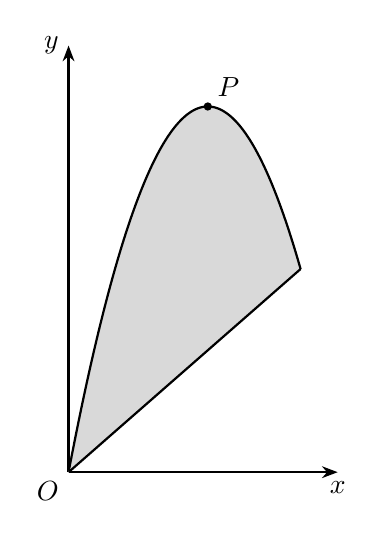
\begin{tikzpicture}
\def\coeff{6}
\def\slope{1}
\pgfmathsetmacro{\rightbound}{\coeff-\slope}
\pgfmathsetmacro{\px}{\coeff/2}
\pgfmathsetmacro{\py}{\coeff*\px-\px^2}
\pgfmathsetmacro{\xmax}{\rightbound+0.8}
\pgfmathsetmacro{\ymax}{\py+1.5}
\begin{axis}[
  width=5cm, height=7cm,
  axis lines=left,
  axis line style={thick, black, -{Stealth[length=2mm]}},
  xlabel={$x$}, ylabel={$y$},
  xmin=0, xmax=\xmax, ymin=0, ymax=\ymax,
  xtick=\empty, ytick=\empty,
  clip=true, clip mode=individual,
  every axis x label/.style={at={(ticklabel* cs:1)}, anchor=north},
  every axis y label/.style={at={(ticklabel* cs:1)}, anchor=east}
]
\addplot[draw=none, name path=upper, domain=0:\rightbound, samples=150] {\coeff*x-x^2};
\addplot[draw=none, name path=lower, domain=0:\rightbound, samples=2] {\slope*x};
\addplot[gray!30] fill between[of=upper and lower];
\addplot[thick, black, domain=0:\rightbound, samples=150] {\coeff*x-x^2};
\addplot[thick, black, domain=0:\rightbound, samples=2] {\slope*x};
\coordinate (P) at (axis cs:\px,\py);
\fill[black] (P) circle (1.5pt);
\node[above right] at (P) {$P$};
\node[below left] at (axis cs:0,0) {$O$};
\end{axis}
\end{tikzpicture}
\end{figure}


A uniform lamina occupies the region enclosed by the curve $y=6x-x^2$ and the straight line $y=x$. \\
The unit of length on each axis is one centimetre. \\
The diagram above shows the lamina and the point $P(3,9)$ at the maximum of the curve. \\
\begin{enumerate}[label=\textbf{(\alph*)}]
\item Find the area of the lamina and use integration to find the coordinates of its centre of mass. Give your answers in exact form. \marks{5} \\
\item The lamina is freely suspended from $P$ and hangs in equilibrium. \\
Find the acute angle between the vertical and the straight edge of the lamina, giving your answer to the nearest degree. \marks{3} \\
\end{enumerate}

\vspace*{10pt}

\begin{djsSolution}
\begin{enumerate}[label=\textbf{(\alph*)}, start=1]
\item The boundaries intersect where
\[
6x-x^2=x
\quad\Longrightarrow\quad
x(5-x)=0
\quad\Longrightarrow\quad
x=0\text{ or }x=5
\]

Regard the lamina as the region under the parabola for \(0\leq x\leq5\), with the triangle beneath \(y=x\) removed.

For a uniform lamina under a curve, the centre of mass formulae are
\[
A=\int_a^b y\,\mathrm{d}x,\qquad
\bar{x}=\frac{1}{A}\int_a^b xy\,\mathrm{d}x,\qquad
\bar{y}=\frac{1}{2A}\int_a^b y^2\,\mathrm{d}x
\]

Using subscript \(1\) for the region under the parabola:
\begin{align*}
A_1&=\int_0^5(6x-x^2)\,\mathrm{d}x
=\left[3x^2-\frac{x^3}{3}\right]_0^5
=\frac{100}{3}\,\mathrm{cm^2}\\
A_1\bar{x}_1&=\int_0^5(6x^2-x^3)\,\mathrm{d}x
=\left[2x^3-\frac{x^4}{4}\right]_0^5
=\frac{375}{4}\,\mathrm{cm^3}\\
A_1\bar{y}_1&=\frac12\int_0^5(36x^2-12x^3+x^4)\,\mathrm{d}x\\
&=\frac12\left[12x^3-3x^4+\frac{x^5}{5}\right]_0^5
=125\,\mathrm{cm^3}
\end{align*}

The removed triangle has vertices \((0,0)\), \((5,0)\) and \((5,5)\). Its centroid coordinates are the means of the vertex coordinates, so
\[
A_2=\frac12(5)(5)=\frac{25}{2}\,\mathrm{cm^2},\qquad
\bar{x}_2=\frac{0+5+5}{3}=\frac{10}{3}\,\mathrm{cm},\qquad
\bar{y}_2=\frac{0+0+5}{3}=\frac53\,\mathrm{cm}
\]

Hence the area of the lamina is
\[
A=A_1-A_2=\frac{100}{3}-\frac{25}{2}=\frac{125}{6}\,\mathrm{cm^2}
\]

For a uniform lamina made of pieces, the centre of mass formulae are
\[
\bar{x}=\dfrac{\sum A_i\bar{x}_i}{\sum A_i},\qquad
\bar{y}=\dfrac{\sum A_i\bar{y}_i}{\sum A_i}
\]

with the area of a removed piece counted as negative. Here this gives
\[
\bar{x}=\frac{A_1\bar{x}_1-A_2\bar{x}_2}{A_1-A_2},\qquad
\bar{y}=\frac{A_1\bar{y}_1-A_2\bar{y}_2}{A_1-A_2}
\]

Therefore
\begin{align*}
\bar{x}&=\frac{\frac{375}{4}-\frac{25}{2}\times\frac{10}{3}}{\frac{125}{6}}
=\frac{\frac{625}{12}}{\frac{125}{6}}
=\frac52\,\mathrm{cm}\\
\bar{y}&=\frac{125-\frac{25}{2}\times\frac53}{\frac{125}{6}}
=\frac{\frac{625}{6}}{\frac{125}{6}}
=5\,\mathrm{cm}
\end{align*}

The centre of mass is \(G\left(\frac52,5\right)\), with coordinates in centimetres.

\item In equilibrium, the centre of mass \(G\) lies vertically below the suspension point \(P\). Thus the required angle is the acute angle between \(PG\) and the straight edge.

In the orientation shown in the question, let \(\phi\) be the acute angle between \(PG\) and a vertical line. Using the horizontal and vertical separations of \(P\) and \(G\):
\[
\tan\phi=\frac{3-\frac52}{9-5}=\frac18
\]

The straight edge \(y=x\) makes an angle of \(45^\circ\) with the vertical. Both it and \(PG\) lean to the same side of the downward vertical, so the required acute angle is
\[
\theta=45^\circ-\arctan\left(\frac18\right)
\approx38^\circ\qquad\text{(nearest degree)}
\]

\end{enumerate}
\end{djsSolution}

\newpage

% ---- Question 2 ----
\questionitem
% [Source: _QBT___Solns__Centre_of_Mass_of_Laminae_by_Integration, Q2]

\begin{figure}[H]
    \centering
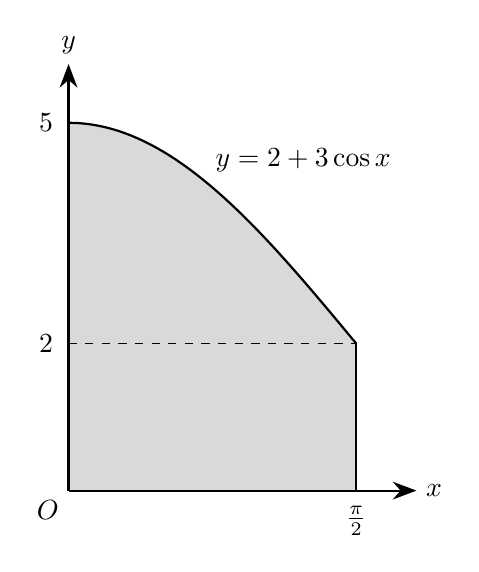
\begin{tikzpicture}
\def\baseheight{2}
\def\amplitude{3}
\pgfmathsetmacro{\rightbound}{pi/2}
\begin{axis}[
  width=6cm, height=7cm,
  axis lines=left,
  axis line style={thick, -{Stealth[length=3mm]}},
  xmin=0, xmax=1.9, ymin=0, ymax=5.8,
  xlabel={$x$}, ylabel={$y$},
  xtick={\rightbound}, xticklabels={$\frac{\pi}{2}$},
  ytick={2,5},
  tick style={draw=none},
  every axis x label/.style={at={(rel axis cs:1,0)},anchor=west},
  every axis y label/.style={at={(rel axis cs:0,1)},anchor=south},
  axis on top,
  clip=true,
  clip mode=individual
]
\addplot[draw=none, fill=gray!30, domain=0:\rightbound, samples=150] {\baseheight+\amplitude*cos(deg(x))} \closedcycle;
\addplot[thick, black, domain=0:\rightbound, samples=150] {\baseheight+\amplitude*cos(deg(x))};
\draw[thick, black] (axis cs:\rightbound,0) -- (axis cs:\rightbound,\baseheight);
\draw[dashed, black] (axis cs:0,\baseheight) -- (axis cs:\rightbound,\baseheight);
\node[above right] at (axis cs:0.75,{\baseheight+\amplitude*cos(deg(0.75))}) {$y=2+3\cos x$};
\node[below left] at (axis cs:0,0) {$O$};
\end{axis}
\end{tikzpicture}
\end{figure}


A uniform lamina $L$ is cut to form a decorative panel. \\
It occupies the region bounded by the curve $y=2+3\cos x$, the $x$-axis and the vertical lines $x=0$ and $x=\frac{\pi}{2}$, as shown in the diagram above. \\
Its centre of mass is $(\bar{x},\bar{y})$. \\

\begin{enumerate}[label=\textbf{(\alph*)}]
  \item Using integration, show that
  \[
  \bar{x}=\dfrac{\pi^2+6\pi-12}{4(\pi+3)}
  \] \marks[-30pt]{2}
  \item Find the exact value of $\bar{y}$. Hence show, without using decimal approximations, that the centre of mass lies above the line $y=2$. \marks{3} \\
\end{enumerate}

\vspace*{10pt}

\begin{djsSolution}
\begin{enumerate}[label=\textbf{(\alph*)}, start=1]
\item For a uniform lamina under a curve, the centre of mass formulae are
\[
A=\int_a^b y\,\mathrm{d}x,
\qquad
\bar{x}=\frac{1}{A}\int_a^b xy\,\mathrm{d}x
\]

Here the area is
\[
A=\int_0^{\pi/2}(2+3\cos x)\,\mathrm{d}x
=\left[2x+3\sin x\right]_0^{\pi/2}
=\pi+3
\]

For the term involving \(x\cos x\), use integration by parts with \(u=x\) and \(\frac{\mathrm{d}v}{\mathrm{d}x}=\cos x\), so \(\frac{\mathrm{d}u}{\mathrm{d}x}=1\) and \(v=\sin x\). This gives
\begin{align*}
\int_0^{\pi/2}x(2+3\cos x)\,\mathrm{d}x
&=\left[x^2+3x\sin x+3\cos x\right]_0^{\pi/2}\\
&=\frac{\pi^2}{4}+\frac{3\pi}{2}-3
\end{align*}

Dividing by the area:
\[
\bar{x}
=\frac{\frac{\pi^2}{4}+\frac{3\pi}{2}-3}{\pi+3}
=\dfrac{\pi^2+6\pi-12}{4(\pi+3)}
\]

\item For a uniform lamina under a curve, the centre of mass formula is
\[
\bar{y}=\frac{1}{2A}\int_a^b y^2\,\mathrm{d}x
\]

Using \(A=\pi+3\) from part (a) and \(\cos^2x=\frac{1+\cos 2x}{2}\):
\begin{align*}
\bar{y}
&=\frac{1}{2(\pi+3)}\int_0^{\pi/2}(2+3\cos x)^2\,\mathrm{d}x\\
&=\frac{1}{2(\pi+3)}\int_0^{\pi/2}\left(4+12\cos x+9\cos^2x\right)\,\mathrm{d}x\\
&=\frac{1}{2(\pi+3)}\int_0^{\pi/2}\left(\frac{17}{2}+12\cos x+\frac{9}{2}\cos 2x\right)\,\mathrm{d}x\\
&=\frac{1}{2(\pi+3)}\left[\frac{17x}{2}+12\sin x+\frac{9}{4}\sin 2x\right]_0^{\pi/2}\\
&=\frac{\frac{17\pi}{4}+12}{2(\pi+3)}
=\dfrac{17\pi+48}{8(\pi+3)}
\end{align*}

The centre of mass lies above the line \(y=2\), since
\[
\bar{y}-2
=\frac{17\pi+48-16(\pi+3)}{8(\pi+3)}
=\frac{\pi}{8(\pi+3)}>0
\]

\end{enumerate}
\end{djsSolution}

\newpage

% ---- Question 3 ----
\questionitem
% [Source: _QBT___Solns__Centre_of_Mass_of_Laminae_by_Integration, Q3]

\begin{figure}[H]
    \centering
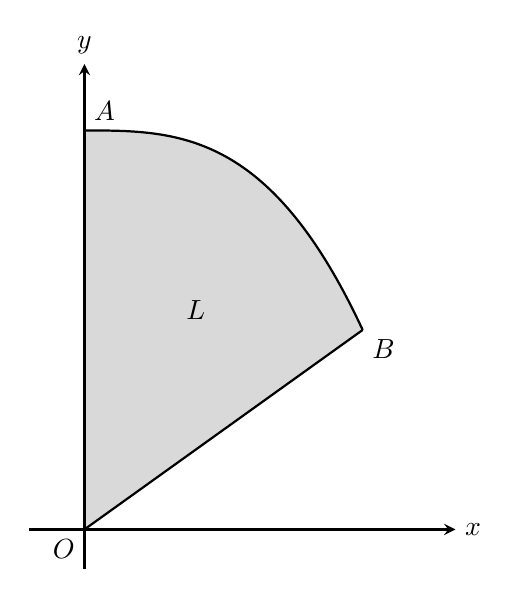
\begin{tikzpicture}
\def\xb{3}
\def\height{6}
\def\denom{9}
\pgfmathsetmacro{\yb}{\height-\xb^3/\denom}
\begin{axis}[
axis lines=center,
axis on top,
xlabel={$x$}, ylabel={$y$},
xmin=-0.6, xmax=4,
ymin=-0.6, ymax=7,
xtick=\empty, ytick=\empty,
width=7cm, height=8cm,
clip=true,
axis line style={thick, black},
every axis x label/.style={at={(ticklabel* cs:1)}, anchor=west},
every axis y label/.style={at={(ticklabel* cs:1)}, anchor=south}
]
\addplot[draw=none, name path=upper, domain=0:\xb, samples=150] {\height-x^3/\denom};
\addplot[draw=none, name path=lower, domain=0:\xb, samples=2] {x};
\addplot[gray!30] fill between[of=upper and lower];
\addplot[thick, black, domain=0:\xb, samples=150] {\height-x^3/\denom};
\addplot[thick, black, domain=0:\xb, samples=2] {x};
\coordinate (O) at (axis cs:0,0);
\coordinate (A) at (axis cs:0,\height);
\coordinate (B) at (axis cs:\xb,\yb);
\draw[thick, black] (O)--(A);
\node[below left] at (O) {$O$};
\node[above right] at (A) {$A$};
\node[below right] at (B) {$B$};
\node at (axis cs:{0.4*\xb},{0.55*\height}) {$L$};
\end{axis}
\end{tikzpicture}
\end{figure}


The diagram above shows a region bounded by the $y$-axis, the straight line $y=x$ and the curve
\[
y=6-\dfrac{x^3}{9}
\] \\
The curve meets the $y$-axis at $A=(0,6)$ and meets the line $y=x$ at $B=(3,3)$. \\
The origin is $O$. \\

A uniform lamina $L$ occupies the shaded region $OAB$. \\
The unit of length on each axis is one centimetre, and its centre of mass has coordinates $(\bar{x},\bar{y})$. \\
\begin{enumerate}[label=\textbf{(\alph*)}]
\item Use integration to find the area of $L$ and show that
\[
\bar{y}=\dfrac{118}{35}
\] \marks[-30pt]{5}
\item The lamina is freely suspended from $B$ and hangs in equilibrium. Find the acute angle between the straight edge $OB$ and the downward vertical, giving your answer in degrees to one decimal place. \marks{8} \\
\end{enumerate}

\vspace*{10pt}

\begin{djsSolution}
\begin{enumerate}[label=\textbf{(\alph*)}, start=1]
\item
Let \(R\) be the region under the curve and above the \(x\)-axis for \(0\leq x\leq3\), and let \(T\) be the triangle with vertices \(O\), \((3,0)\) and \(B\). The lamina \(L\) is obtained by removing \(T\) from \(R\).

For a uniform lamina under a curve, the centre of mass formulae are
\[
\mathcal{A}=\int_a^b y\,\mathrm{d}x,
\qquad
\bar{y}=\frac{1}{2\mathcal{A}}\int_a^b y^2\,\mathrm{d}x
\]

The areas are
\begin{align*}
\mathcal{A}_R&=\int_0^3\left(6-\frac{x^3}{9}\right)\,\mathrm{d}x
=\left[6x-\frac{x^4}{36}\right]_0^3
=\frac{63}{4}\,\mathrm{cm^2}\\
\mathcal{A}_T&=\frac12\times3\times3=\frac92\,\mathrm{cm^2}\\
\mathcal{A}_L&=\mathcal{A}_R-\mathcal{A}_T=\frac{63}{4}-\frac92=\frac{45}{4}\,\mathrm{cm^2}
\end{align*}

Writing the centre of mass of \(R\) as \((\bar{x}_R,\bar{y}_R)\), we obtain
\begin{align*}
\bar{y}_R
&=\frac{1}{2(63/4)}\int_0^3\left(6-\frac{x^3}{9}\right)^2\,\mathrm{d}x\\
&=\frac{2}{63}\int_0^3\left(36-\frac{4x^3}{3}+\frac{x^6}{81}\right)\,\mathrm{d}x\\
&=\frac{2}{63}\left[36x-\frac{x^4}{3}+\frac{x^7}{567}\right]_0^3
=\frac{132}{49}\,\mathrm{cm}
\end{align*}

The centroid of \(T\) has coordinates equal to the means of its vertex coordinates, so
\[
\bar{y}_T=\frac{0+0+3}{3}=1\,\mathrm{cm}
\]

For a uniform lamina made of pieces, the centre of mass formula is
\[
\bar{y}=\dfrac{\sum\mathcal{A}_i\bar{y}_i}{\sum\mathcal{A}_i}
\]

with the area of a removed piece counted as negative. Hence
\begin{align*}
\bar{y}
&=\frac{\mathcal{A}_R\bar{y}_R-\mathcal{A}_T\bar{y}_T}{\mathcal{A}_R-\mathcal{A}_T}\\
&=\frac{\frac{63}{4}\times\frac{132}{49}-\frac92\times1}{\frac{45}{4}}
=\frac{118}{35}\,\mathrm{cm}
\end{align*}

\item
We first find \(\bar{x}\). For a uniform lamina under a curve, the centre of mass formula is
\[
\bar{x}=\frac{1}{\mathcal{A}}\int_a^b xy\,\mathrm{d}x
\]

Applying this to \(R\):
\begin{align*}
\bar{x}_R
&=\frac{1}{63/4}\int_0^3 x\left(6-\frac{x^3}{9}\right)\,\mathrm{d}x\\
&=\frac{4}{63}\left[3x^2-\frac{x^5}{45}\right]_0^3
=\frac{48}{35}\,\mathrm{cm}
\end{align*}

For the triangle \(T\), averaging the vertex coordinates gives
\[
\bar{x}_T=\frac{0+3+3}{3}=2\,\mathrm{cm}
\]

For a uniform lamina made of pieces, the centre of mass formula is
\[
\bar{x}=\dfrac{\sum\mathcal{A}_i\bar{x}_i}{\sum\mathcal{A}_i}
\]

with the area of a removed piece counted as negative. Hence
\begin{align*}
\bar{x}
&=\frac{\mathcal{A}_R\bar{x}_R-\mathcal{A}_T\bar{x}_T}{\mathcal{A}_R-\mathcal{A}_T}\\
&=\frac{\frac{63}{4}\times\frac{48}{35}-\frac92\times2}{\frac{45}{4}}
=\frac{28}{25}\,\mathrm{cm}
\end{align*}

Thus the centre of mass is \(G\left(\frac{28}{25},\frac{118}{35}\right)\). When the lamina hangs in equilibrium, \(G\) lies vertically below the suspension point \(B\). The required angle is therefore \(\angle OBG\).

In the original diagram, \(G\) is to the left of and above \(B(3,3)\). Let \(\phi\) be the acute angle between \(BG\) and the leftward horizontal through \(B\). Then
\begin{align*}
\tan\phi
&=\frac{\bar{y}-3}{3-\bar{x}}\\
&=\frac{\frac{118}{35}-3}{3-\frac{28}{25}}
=\frac{65}{329}\\
\phi&=\arctan\left(\frac{65}{329}\right)
\end{align*}

Since \(OB\) lies on \(y=x\), the direction from \(B\) towards \(O\) is \(45^\circ\) below the leftward horizontal. Hence the required acute angle is
\[
\angle OBG=45^\circ+\phi\approx56.2^\circ
\qquad\text{(1 d.p.)}
\]

\end{enumerate}
\end{djsSolution}

\newpage

% ---- Question 4 ----
\questionitem
% [Source: _QBT___Solns__Centre_of_Mass_of_Laminae_by_Integration, Q4]

\begin{figure}[H]
    \centering
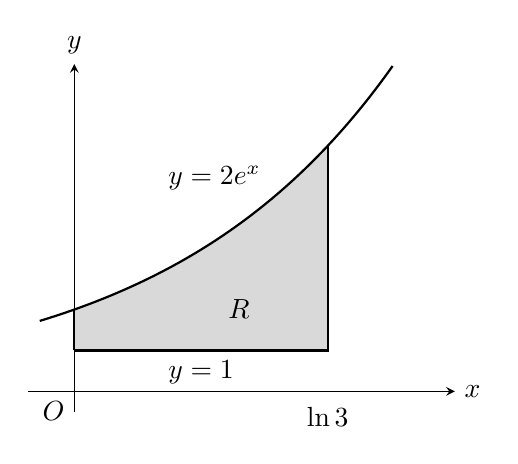
\begin{tikzpicture}
\def\coeff{2}
\def\base{1}
\pgfmathsetmacro{\rightx}{ln(3)}
\begin{axis}[
  width=7cm,height=6cm,
  axis lines=center,axis on top,
  xlabel={$x$},ylabel={$y$},
  xmin=-0.2,xmax=1.65,ymin=-0.5,ymax=8,
  xtick={\rightx},xticklabels={$\ln 3$},
  ytick=\empty,tick style={draw=none},
  clip=true,clip mode=individual,
  every axis x label/.style={at={(ticklabel* cs:1)},anchor=west},
  every axis y label/.style={at={(ticklabel* cs:1)},anchor=south}
]
\addplot[draw=none,name path=upper,domain=0:\rightx,samples=120] {\coeff*exp(x)};
\addplot[draw=none,name path=lower,domain=0:\rightx,samples=2] {\base};
\addplot[gray!30] fill between[of=upper and lower];
\addplot[thick,black,domain=-0.15:1.38,samples=150] {\coeff*exp(x)};
\draw[thick,black] (axis cs:0,\base) -- (axis cs:\rightx,\base) -- (axis cs:\rightx,{\coeff*exp(\rightx)});
\draw[thick,black] (axis cs:0,\base) -- (axis cs:0,\coeff);
\node[above left] at (axis cs:0.85,{\coeff*exp(0.85)}) {$y=2e^x$};
\node[below] at (axis cs:{\rightx/2},\base) {$y=1$};
\node at (axis cs:{0.65*\rightx},2) {$R$};
\node[below left] at (axis cs:0,0) {$O$};
\end{axis}
\end{tikzpicture}
\end{figure}


\begin{figure}[H]
    \centering
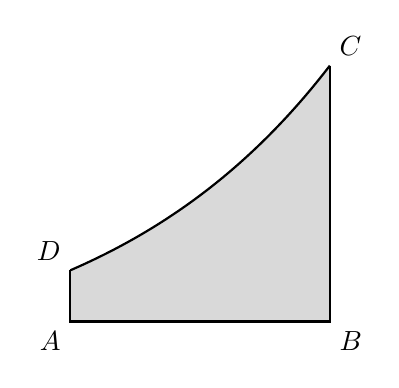
\begin{tikzpicture}[x=3cm,y=0.65cm]
\def\coeff{2}
\def\base{1}
\pgfmathsetmacro{\widthAB}{ln(3)}
\pgfmathsetmacro{\heightC}{\coeff*exp(\widthAB)}
\coordinate (A) at (0,\base);
\coordinate (B) at (\widthAB,\base);
\coordinate (C) at (\widthAB,\heightC);
\coordinate (D) at (0,\coeff);
\fill[gray!30] (A) -- (B) -- (C) -- plot[domain=\widthAB:0,samples=120] (\x,{\coeff*exp(\x)}) -- cycle;
\draw[thick,black] (D) -- (A) -- (B) -- (C);
\draw[thick,black] plot[domain=0:\widthAB,samples=120] (\x,{\coeff*exp(\x)});
\node[below left] at (A) {$A$};
\node[below right] at (B) {$B$};
\node[above right] at (C) {$C$};
\node[above left] at (D) {$D$};
\end{tikzpicture}
\end{figure}


The shaded region $R$ is bounded by the curve $y=2e^x$, the horizontal line $y=1$, the $y$-axis and the line $x=\ln 3$. \\
The unit of length on each axis is one metre. \\

A uniform lamina occupies $R$, and its centre of mass has coordinates $(\bar{x},\bar{y})$. \\
\begin{enumerate}[label=\textbf{(\alph*)}]
\item Use integration to find the area of $R$ and show that
\[
\bar{y}=\dfrac{16-\ln 3}{8-2\ln 3}
\] \marks[-30pt]{5}
\end{enumerate}
The second diagram above shows the same lamina, with vertices $A=(0,1)$, $B=(\ln 3,1)$, $C=(\ln 3,6)$ and $D=(0,2)$. \\

The lamina is freely suspended from $D$ and hangs in equilibrium. \\
Let $\theta$ be the angle between the directed segment from $D$ to $A$ and the downward vertical, where $0^\circ\leq\theta\leq180^\circ$. \\
\begin{enumerate}[label=\textbf{(\alph*)}, resume]
\item Use integration to find $\bar{x}$ in exact form. Hence find $\theta$, giving your answer to one decimal place. \marks{7} \\
\end{enumerate}

\vspace*{10pt}

\begin{djsSolution}
\begin{enumerate}[label=\textbf{(\alph*)}, start=1]
\item Regard \(R\) as the region \(S\) beneath \(y=2e^x\) and above the \(x\)-axis, for \(0\leq x\leq\ln3\), with the rectangle \(T\) of height \(1\) removed.

For a uniform lamina under a curve, the centre of mass formulae are
\[
\mathcal{A}=\int_a^b y\,\mathrm{d}x,
\qquad
\bar{y}=\frac{1}{2\mathcal{A}}\int_a^b y^2\,\mathrm{d}x
\]

The areas of \(S\), \(T\) and \(R\) are therefore
\begin{align*}
\mathcal{A}_S&=\int_0^{\ln3}2e^x\,\mathrm{d}x
=\left[2e^x\right]_0^{\ln3}=4\,\mathrm{m^2}\\
\mathcal{A}_T&=\ln3\,\mathrm{m^2}\\
\mathcal{A}&=\mathcal{A}_S-\mathcal{A}_T=(4-\ln3)\,\mathrm{m^2}
\end{align*}

The vertical coordinate of the centre of mass of \(S\) is
\begin{align*}
\bar{y}_S
&=\frac{1}{2(4)}\int_0^{\ln3}4e^{2x}\,\mathrm{d}x\\
&=\frac18\left[2e^{2x}\right]_0^{\ln3}
=2\,\mathrm{m}
\end{align*}

The rectangle has \(\bar{y}_T=\frac12\,\mathrm{m}\). For a uniform lamina made of pieces, the centre of mass formula is
\[
\bar{y}=\dfrac{\sum\mathcal{A}_i\bar{y}_i}{\sum\mathcal{A}_i}
\]

with the area of a removed piece counted as negative. Hence
\begin{align*}
\bar{y}
&=\frac{\mathcal{A}_S\bar{y}_S-\mathcal{A}_T\bar{y}_T}{\mathcal{A}_S-\mathcal{A}_T}\\
&=\frac{4(2)-(\ln3)\left(\frac12\right)}{4-\ln3}\\
&=\frac{16-\ln3}{8-2\ln3}\,\mathrm{m}
\end{align*}

\item For a uniform lamina under a curve, the centre of mass formula is
\[
\bar{x}=\frac{1}{\mathcal{A}}\int_a^b xy\,\mathrm{d}x
\]

For \(S\), integrate by parts, taking \(u=x\) and \(\frac{\mathrm{d}v}{\mathrm{d}x}=2e^x\), so that \(\frac{\mathrm{d}u}{\mathrm{d}x}=1\) and \(v=2e^x\):
\begin{align*}
\mathcal{A}_S\bar{x}_S
&=\int_0^{\ln3}2xe^x\,\mathrm{d}x\\
&=\left[2xe^x\right]_0^{\ln3}-\int_0^{\ln3}2e^x\,\mathrm{d}x\\
&=\left[2(x-1)e^x\right]_0^{\ln3}\\
&=(6\ln3-4)\,\mathrm{m^3}
\end{align*}

The rectangle has \(\bar{x}_T=\frac{\ln3}{2}\,\mathrm{m}\). For a uniform lamina made of pieces, the centre of mass formula is
\[
\bar{x}=\dfrac{\sum\mathcal{A}_i\bar{x}_i}{\sum\mathcal{A}_i}
\]

with the area of a removed piece counted as negative. Hence
\begin{align*}
\bar{x}
&=\frac{\mathcal{A}_S\bar{x}_S-\mathcal{A}_T\bar{x}_T}{\mathcal{A}_S-\mathcal{A}_T}\\
&=\frac{6\ln3-4-\frac12(\ln3)^2}{4-\ln3}\\
&=\frac{12\ln3-8-(\ln3)^2}{8-2\ln3}\,\mathrm{m}
\end{align*}

Let \(G\) be the centre of mass. In equilibrium, \(G\) lies vertically below the suspension point \(D\), so \(\theta\) is the angle between the directed segments \(DA\) and \(DG\).

In the original orientation, \(\bar{x}>0\), and part (a) gives
\[
\bar{y}-2
=\frac{16-\ln3-2(8-2\ln3)}{8-2\ln3}
=\frac{3\ln3}{8-2\ln3}>0
\]

Thus \(G\) is above and to the right of \(D\), whereas \(DA\) points downwards. Hence \(\theta\) is obtuse, and the right-angled triangle formed by the horizontal and vertical displacements from \(D\) to \(G\) gives
\begin{align*}
\tan(180^\circ-\theta)
&=\frac{\bar{x}}{\bar{y}-2}\\
&=\frac{12\ln3-8-(\ln3)^2}{3\ln3}\\
\theta
&=180^\circ-\arctan\left(\frac{12\ln3-8-(\ln3)^2}{3\ln3}\right)\\
&\approx129.7^\circ\qquad\text{(1 d.p.)}
\end{align*}

\end{enumerate}
\end{djsSolution}

\newpage

% ---- Question 5 ----
\questionitem
% [Source: _QBT___Solns__Centre_of_Mass_of_Laminae_by_Integration, Q5]

A uniform lamina occupies the region bounded by the curve
\[
y=\dfrac{k}{x+1}
\] \\
the $x$-axis and the vertical lines $x=0$ and $x=3$, where $k$ is a positive constant. \\

\begin{enumerate}[label=\textbf{(\roman*)}]
  \item Find the exact $x$-coordinate of the centre of mass of the lamina. \marks{6} \\
  \item The centre of mass lies on the line $y=x$. \\
  Find the exact value of $k$ and hence the exact area of the lamina. \marks{5} \\
\end{enumerate}

\vspace*{10pt}

\begin{djsSolution}
\begin{enumerate}[label=\textbf{(\roman*)}, start=1]
\item A schematic diagram of the lamina is:\par\nopagebreak

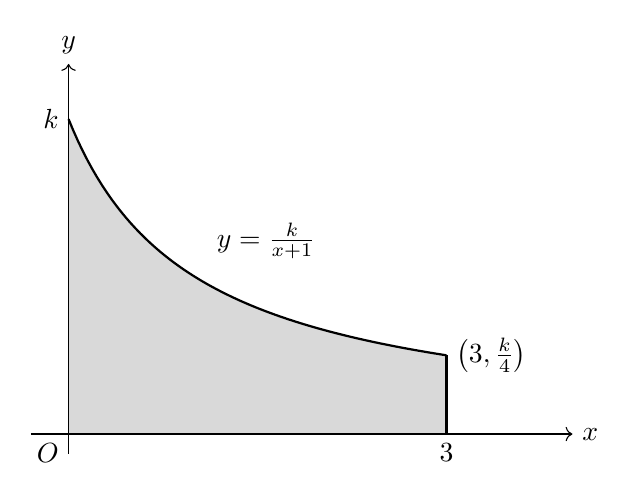
\begin{tikzpicture}[x=1.6cm,y=1cm]
  \fill[gray!30] (0,0) -- plot[domain=0:3,samples=80] (\x,{4/(\x+1)}) -- (3,0) -- cycle;
  \draw[->] (-0.3,0) -- (4,0) node[right] {$x$};
  \draw[->] (0,-0.25) -- (0,4.7) node[above] {$y$};
  \draw[thick,domain=0:3,samples=80] plot (\x,{4/(\x+1)});
  \draw[thick] (3,0) -- (3,1);
  \node[below left] at (0,0) {$O$};
  \node[left] at (0,4) {$k$};
  \node[below] at (3,0) {$3$};
  \node[right] at (3,1) {$\left(3,\frac{k}{4}\right)$};
  \node[above right] at (1.1,2.1) {$y=\frac{k}{x+1}$};
\end{tikzpicture}

For a uniform lamina under a curve, the centre of mass formulae are
\[
A=\int_a^b y\,\mathrm{d}x,
\qquad
\bar{x}=\frac{1}{A}\int_a^b xy\,\mathrm{d}x
\]

The area of this lamina is
\begin{align*}
A&=\int_0^3 \dfrac{k}{x+1}\,\mathrm{d}x\\
&=k\left[\ln(x+1)\right]_0^3\\
&=k\ln4
\end{align*}

Using \(\frac{x}{x+1}=1-\frac{1}{x+1}\):
\begin{align*}
\int_0^3 xy\,\mathrm{d}x
&=k\int_0^3\dfrac{x}{x+1}\,\mathrm{d}x\\
&=k\int_0^3\left(1-\dfrac{1}{x+1}\right)\,\mathrm{d}x\\
&=k\left[x-\ln(x+1)\right]_0^3\\
&=k(3-\ln4)
\end{align*}

Therefore
\[
\bar{x}=\dfrac{k(3-\ln4)}{k\ln4}
=\dfrac{3-\ln4}{\ln4}
\]

\item For a uniform lamina under a curve, the centre of mass formula is
\[
\bar{y}=\frac{1}{2A}\int_a^b y^2\,\mathrm{d}x
\]

Using \(A=k\ln4\) from part (i):
\begin{align*}
\bar{y}
&=\dfrac{1}{2k\ln4}\int_0^3\dfrac{k^2}{(x+1)^2}\,\mathrm{d}x\\
&=\dfrac{k}{2\ln4}\left[-\dfrac{1}{x+1}\right]_0^3\\
&=\dfrac{k}{2\ln4}\left(1-\dfrac14\right)\\
&=\dfrac{3k}{8\ln4}
\end{align*}

Since the centre of mass lies on \(y=x\), we have \(\bar{y}=\bar{x}\). Thus
\begin{align*}
\dfrac{3k}{8\ln4}&=\dfrac{3-\ln4}{\ln4}\\
3k&=8(3-\ln4)\\
k&=\dfrac{8(3-\ln4)}{3}
\end{align*}

Hence the exact area is
\[
A=k\ln4=\dfrac{8(3-\ln4)\ln4}{3}
\]

\end{enumerate}
\end{djsSolution}

\newpage

% ---- Question 6 ----
\questionitem
% [Source: _QBT___Solns__Centre_of_Mass_of_Laminae_by_Integration, Q6]

\begin{figure}[H]
    \centering
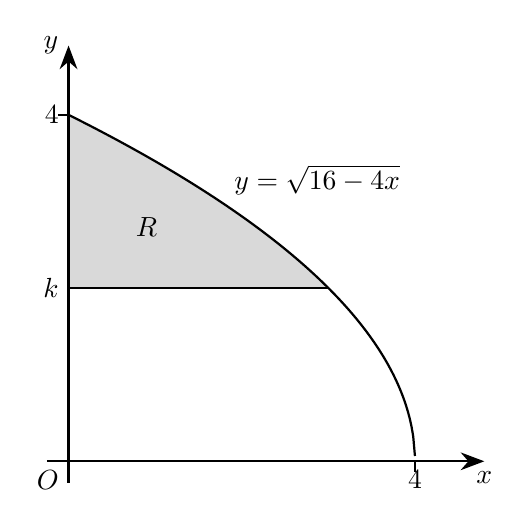
\begin{tikzpicture}[scale=1.1]
\def\height{4}
\def\coeff{4}
\def\kval{2}
\def\margin{0.8}
\def\ticklen{0.12}
\pgfmathsetmacro{\endx}{\height*\height/\coeff}
\pgfmathsetmacro{\cutx}{(\height*\height-\kval*\kval)/\coeff}
\coordinate (O) at (0,0);
\coordinate (Y) at (0,\height);
\coordinate (X) at (\endx,0);
\coordinate (K) at (0,\kval);
\coordinate (P) at (\cutx,\kval);
\coordinate (CLabel) at ({0.45*\endx},{sqrt(\height*\height-\coeff*0.45*\endx)});
\coordinate (RLabel) at ({0.3*\cutx},{\kval+0.35*(\height-\kval)});
\fill[gray!30] (K) -- (P) -- plot[domain=\cutx:0,samples=150] (\x,{sqrt(max(0,\height*\height-\coeff*\x))}) -- cycle;
\draw[thick,black,-{Stealth[length=3mm]}] (-0.25,0) -- ({\endx+\margin},0) node[below] {$x$};
\draw[thick,black,-{Stealth[length=3mm]}] (0,-0.25) -- (0,{\height+\margin}) node[left] {$y$};
\draw[thick,black,domain=0:\endx,samples=200] plot (\x,{sqrt(max(0,\height*\height-\coeff*\x))});
\draw[thick,black] (K) -- (P);
\draw[thick,black] ($(Y)+(-\ticklen,0)$) -- (Y);
\draw[thick,black] ($(X)+(0,-\ticklen)$) -- (X);
\node[below left] at (O) {$O$};
\node[left] at (Y) {$4$};
\node[below] at (X) {$4$};
\node[left] at (K) {$k$};
\node[above right] at (CLabel) {$y=\sqrt{16-4x}$};
\node at (RLabel) {$R$};
\end{tikzpicture}
\end{figure}


The shaded region $R$ is bounded by the curve $y=\sqrt{16-4x}$, the $y$-axis and the horizontal line $y=k$, where $0<k<4$. \\
A uniform lamina occupies $R$. \\
\begin{enumerate}[label=\textbf{(\alph*)}]
\item Using integration, determine the $y$-coordinate of the centre of mass of the lamina in terms of $k$. Simplify your expression fully. \marks{6} \\
\item The centre of mass lies on the line $y=3$. Find the exact value of $k$, explaining why any other root of your equation must be rejected. \marks{3} \\
\end{enumerate}

\vspace*{10pt}

\begin{djsSolution}
\begin{enumerate}[label=\textbf{(\alph*)}, start=1]
\item Rearranging the curve equation to express \(x\) in terms of \(y\) gives
\[
x=4-\frac{y^2}{4}
\]

For a uniform lamina against the \(y\)-axis, the centre of mass formulae are
\[
A=\int_a^b x\,\mathrm{d}y,
\qquad
\bar{y}=\frac{1}{A}\int_a^b xy\,\mathrm{d}y
\]

The area is therefore
\begin{align*}
A&=\int_k^4\left(4-\frac{y^2}{4}\right)\,\mathrm{d}y\\
&=\left[4y-\frac{y^3}{12}\right]_k^4\\
&=\frac{32}{3}-4k+\frac{k^3}{12}\\
&=\frac{k^3-48k+128}{12}
\end{align*}

Using the centre of mass formula:
\begin{align*}
A\bar{y}&=\int_k^4 y\left(4-\frac{y^2}{4}\right)\,\mathrm{d}y\\
&=\left[2y^2-\frac{y^4}{16}\right]_k^4\\
&=16-2k^2+\frac{k^4}{16}\\
&=\frac{(k^2-16)^2}{16}
\end{align*}

Dividing by \(A\), factorising and cancelling \((k-4)^2\), which is non-zero since \(0<k<4\), gives
\begin{align*}
\bar{y}
&=\frac{3(k^2-16)^2}{4(k^3-48k+128)}\\
&=\frac{3(k-4)^2(k+4)^2}{4(k-4)^2(k+8)}\\
&=\frac{3(k+4)^2}{4(k+8)}
\end{align*}

\item Since the centre of mass lies on \(y=3\), part (a) gives
\begin{align*}
\frac{3(k+4)^2}{4(k+8)}&=3\\
(k+4)^2&=4(k+8)\\
k^2+4k-16&=0\\
(k+2)^2&=20\\
k&=-2\pm2\sqrt{5}
\end{align*}

The root \(-2-2\sqrt{5}\) is negative, so it is rejected because \(0<k<4\). The other root lies between \(0\) and \(4\), so
\[
k=2(\sqrt{5}-1)
\]

\end{enumerate}
\end{djsSolution}

\newpage

% ---- Question 7 ----
\questionitem
% [Source: _QBT___Solns__Centre_of_Mass_of_Laminae_by_Integration, Q7]

A uniform lamina occupies the region between the curve $y=4e^{-x/2}$ and the line $y=1$, for $0\leq x\leq 2\ln 2$. \\
\begin{enumerate}[label=\textbf{(\roman*)}]
\item Using integration, find the exact area of this lamina and the exact $y$-coordinate of its centre of mass. \marks{7} \\
\end{enumerate}

\begin{figure}[H]
    \centering
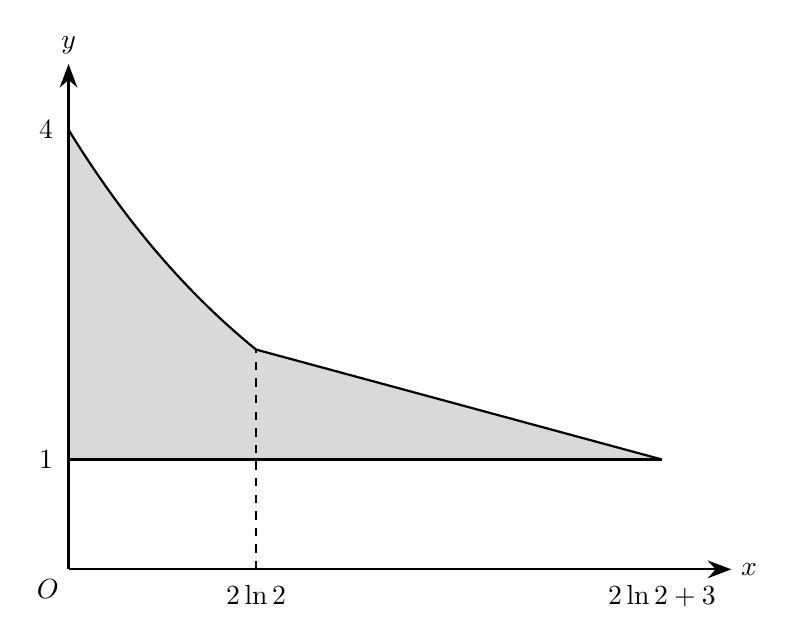
\begin{tikzpicture}
\def\height{4}
\def\baseline{1}
\def\extension{3}
\pgfmathsetmacro{\joinx}{2*ln(2)}
\pgfmathsetmacro{\joiny}{\height*exp(-\joinx/2)}
\pgfmathsetmacro{\endx}{\joinx+\extension}
\begin{axis}[
  width=10cm, height=8cm,
  axis lines=left,
  axis line style={thick, black, -{Stealth[length=3mm]}},
  xlabel={$x$}, ylabel={$y$},
  xmin=0, xmax=4.9, ymin=0, ymax=4.6,
  xtick={\joinx,\endx},
  xticklabels={$2\ln 2$,$2\ln 2+3$},
  ytick={1,4},
  tick style={draw=none},
  grid=none, clip=true, clip mode=individual, axis on top,
  every axis x label/.style={at={(ticklabel* cs:1)}, anchor=west},
  every axis y label/.style={at={(ticklabel* cs:1)}, anchor=south}
]
\addplot[draw=none, name path=upper, samples=150, domain=0:\joinx] {\height*exp(-x/2)};
\addplot[draw=none, name path=lower, samples=2, domain=0:\joinx] {\baseline};
\addplot[gray!30] fill between[of=upper and lower];
\fill[gray!30] (axis cs:\joinx,\baseline) -- (axis cs:\joinx,\joiny) -- (axis cs:\endx,\baseline) -- cycle;
\draw[thick, black] (axis cs:0,\baseline) -- (axis cs:0,\height);
\addplot[thick, black, samples=150, domain=0:\joinx] {\height*exp(-x/2)};
\addplot[thick, black, samples=2, domain=\joinx:\endx] {\joiny-(\joiny-\baseline)*(x-\joinx)/\extension};
\addplot[thick, black, samples=2, domain=0:\endx] {\baseline};
\draw[dashed, thick, black] (axis cs:\joinx,0) -- (axis cs:\joinx,\joiny);
\node[below left] at (axis cs:0,0) {$O$};
\end{axis}
\end{tikzpicture}
\end{figure}


A triangular piece of lamina with the same uniform mass per unit area is attached to its right-hand edge. \\
The resulting lamina is shown in the diagram above. \\
Its lower boundary is $y=1$ and its upper boundary is $y=f(x)$, where
\[
f(x)=\begin{cases}
4e^{-x/2}, & 0\leq x\leq 2\ln 2\\[3pt]
2-\dfrac{x-2\ln 2}{3}, & 2\ln 2\leq x\leq 2\ln 2+3
\end{cases}
\] \\
Its left-hand boundary lies on the $y$-axis. \\
\begin{enumerate}[label=\textbf{(\roman*)}, resume]
\item Using your area from part (i), find the exact $x$-coordinate of the centre of mass of the resulting lamina. \marks{7} \\
\end{enumerate}

\vspace*{10pt}

\begin{djsSolution}
\begin{enumerate}[label=\textbf{(\roman*)}, start=1]
\item Regard the lamina as the region under \(y=4e^{-x/2}\) down to the \(x\)-axis, with a rectangle removed. Denote these two regions by \(C\) and \(R\), respectively.

For a uniform lamina under a curve, the centre of mass formulae are
\[
A=\int_a^b y\,\mathrm{d}x,
\qquad
\bar{y}=\frac{1}{2A}\int_a^b y^2\,\mathrm{d}x
\]

The area of \(C\) is
\begin{align*}
A_C&=\int_0^{2\ln 2}4e^{-x/2}\,\mathrm{d}x\\
&=\left[-8e^{-x/2}\right]_0^{2\ln 2}\\
&=-4+8=4
\end{align*}

The removed rectangle has width \(2\ln 2\) and height \(1\), so the required area is
\[
A=A_C-A_R=4-2\ln 2
\]

Applying the centre of mass formula to \(C\):
\begin{align*}
\bar y_C&=\dfrac{1}{2(4)}\int_0^{2\ln 2}16e^{-x}\,\mathrm{d}x\\
&=\dfrac18\left[-16e^{-x}\right]_0^{2\ln 2}\\
&=\dfrac18(-4+16)=\dfrac32
\end{align*}

The rectangle has \(\bar{y}_R=\frac12\). For a uniform lamina made of pieces, the centre of mass formula is
\[
\bar{y}=\dfrac{\sum A_i\bar{y}_i}{\sum A_i}
\]

with the area of a removed piece counted as negative. Hence
\begin{align*}
\bar y&=\dfrac{A_C\bar y_C-A_R\bar y_R}{A_C-A_R}\\
&=\dfrac{4\left(\frac32\right)-(2\ln 2)\left(\frac12\right)}{4-2\ln 2}\\
&=\dfrac{6-\ln 2}{4-2\ln 2}
\end{align*}

\item First find the horizontal position of the centre of mass of the original lamina, using the same regions \(C\) and \(R\).

For a uniform lamina under a curve, the centre of mass formula is
\[
\bar{x}=\frac{1}{A}\int_a^b xy\,\mathrm{d}x
\]

To integrate \(4xe^{-x/2}\) by parts, take \(u=x\) and \(\frac{\mathrm{d}v}{\mathrm{d}x}=4e^{-x/2}\), so \(\frac{\mathrm{d}u}{\mathrm{d}x}=1\) and \(v=-8e^{-x/2}\). Thus
\begin{align*}
A_C\bar x_C&=\int_0^{2\ln 2}4xe^{-x/2}\,\mathrm{d}x\\
&=\left[-8xe^{-x/2}\right]_0^{2\ln 2}
+8\int_0^{2\ln 2}e^{-x/2}\,\mathrm{d}x\\
&=\left[-8(x+2)e^{-x/2}\right]_0^{2\ln 2}\\
&=-4(2\ln 2+2)+16\\
&=8-8\ln 2
\end{align*}

The rectangle has \(\bar{x}_R=\ln 2\). For a uniform lamina made of pieces, the centre of mass formula is
\[
\bar{x}=\dfrac{\sum A_i\bar{x}_i}{\sum A_i}
\]

with the area of a removed piece counted as negative. Using the area \(A=4-2\ln 2\) from part (i), the original lamina therefore has
\begin{align*}
\bar x_0&=\dfrac{A_C\bar x_C-A_R\bar x_R}{A}\\
&=\dfrac{8-8\ln 2-(2\ln 2)(\ln 2)}{4-2\ln 2}\\
&=\dfrac{8-8\ln 2-2(\ln 2)^2}{4-2\ln 2}
\end{align*}

The attached triangle has base \(3\) and height \(1\). Its centroid's \(x\)-coordinate is the mean of its vertices' \(x\)-coordinates, so
\[
A_T=\dfrac12(3)(1)=\dfrac32,
\qquad
\bar x_T=\dfrac{2\ln 2+2\ln 2+(2\ln 2+3)}{3}=2\ln 2+1
\]

Since both pieces have the same uniform mass per unit area, the same formula applies to the original lamina and the attached triangle:
\begin{align*}
\bar x&=\dfrac{A\bar x_0+A_T\bar x_T}{A+A_T}\\
&=\dfrac{8-8\ln 2-2(\ln 2)^2+\frac32(2\ln 2+1)}{4-2\ln 2+\frac32}\\
&=\dfrac{\frac{19}{2}-5\ln 2-2(\ln 2)^2}{\frac{11}{2}-2\ln 2}\\
&=\dfrac{19-10\ln 2-4(\ln 2)^2}{11-4\ln 2}
\end{align*}

\end{enumerate}
\end{djsSolution}

\newpage

% ---- Question 8 ----
\questionitem
% [Source: _QBT___Solns__Centre_of_Mass_of_Laminae_by_Integration, Q8]

\begin{figure}[H]
    \centering
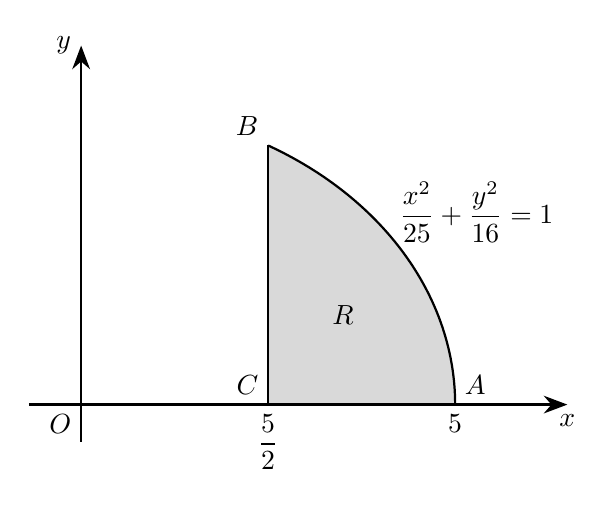
\begin{tikzpicture}[scale=0.95]
\def\a{5}
\def\b{4}
\def\cutfrac{0.5}
\pgfmathsetmacro{\xc}{\a*\cutfrac}
\pgfmathsetmacro{\yb}{\b*sqrt(1-\cutfrac^2)}
\pgfmathsetmacro{\endang}{acos(\cutfrac)}
\coordinate (O) at (0,0);
\coordinate (C) at (\xc,0);
\coordinate (A) at (\a,0);
\coordinate (B) at (\xc,\yb);
\coordinate (E) at ({\a*cos(40)},{\b*sin(40)});
\fill[gray!30] (C) -- (A) -- plot[domain=0:\endang,samples=100] ({\a*cos(\x)},{\b*sin(\x)}) -- cycle;
\draw[thick,black,-{Stealth[length=3mm]}] ({-0.14*\a},0) -- ({1.3*\a},0) node[below] {$x$};
\draw[thick,black,-{Stealth[length=3mm]}] (0,{-0.125*\b}) -- (0,{1.2*\b}) node[left] {$y$};
\draw[thick,black] (C) -- (B);
\draw[thick,black] plot[domain=0:\endang,samples=100] ({\a*cos(\x)},{\b*sin(\x)});
\node[below left] at (O) {$O$};
\node[above left] at (C) {$C$};
\node[below] at (C) {$\dfrac{5}{2}$};
\node[above right] at (A) {$A$};
\node[below] at (A) {$5$};
\node[above left] at (B) {$B$};
\node[right=8pt] at (E) {$\dfrac{x^2}{25}+\dfrac{y^2}{16}=1$};
\node at ($(C)!0.4!(A)+(0,{0.3*\b})$) {$R$};
\end{tikzpicture}
\end{figure}


A uniform lamina occupies the shaded region $R$, bounded by the upper arc of the ellipse
\[
\dfrac{x^2}{25}+\dfrac{y^2}{16}=1
\] \\
the line $x=\frac{5}{2}$ and the $x$-axis. \\

The points $C$ and $A$ have coordinates $\left(\frac{5}{2},0\right)$ and $(5,0)$ respectively. \\
The point $B$ is the upper intersection of the ellipse with $x=\frac{5}{2}$. \\
The unit of length on each axis is one metre. \\
\begin{enumerate}[label=\textbf{(\alph*)}]
\item Using the substitution $x=5\sin t$, show by integration that the area of $R$ is
\[
\dfrac{5}{6}\left(4\pi-3\sqrt{3}\right)\,\mathrm{m}^2
\] \marks[-30pt]{4}
\item Use integration to find the exact coordinates $(\bar{x},\bar{y})$ of the centre of mass of the lamina. \marks{6} \\
\item The lamina is freely suspended from $A$ and hangs in equilibrium. Find the acute angle between $AC$ and the downward vertical, giving your answer in degrees to one decimal place. \marks{3} \\
\end{enumerate}

\vspace*{10pt}

\begin{djsSolution}
\begin{enumerate}[label=\textbf{(\alph*)}, start=1]
\item The upper arc of the ellipse has equation
\[
y=4\sqrt{1-\dfrac{x^2}{25}}
\]

Using the given substitution \(x=5\sin t\), we have \(\mathrm{d}x=5\cos t\,\mathrm{d}t\) and \(y=4\cos t\). The limits \(x=\frac{5}{2}\) and \(x=5\) correspond to \(t=\frac{\pi}{6}\) and \(t=\frac{\pi}{2}\), respectively.

The area \(\mathcal{A}\) is therefore
\begin{align*}
\mathcal{A}&=\int_{5/2}^{5}y\,\mathrm{d}x\\
&=20\int_{\pi/6}^{\pi/2}\cos^2t\,\mathrm{d}t\\
&=10\int_{\pi/6}^{\pi/2}(1+\cos 2t)\,\mathrm{d}t\\
&=10\left[t+\dfrac{1}{2}\sin 2t\right]_{\pi/6}^{\pi/2}\\
&=\dfrac{10\pi}{3}-\dfrac{5\sqrt{3}}{2}\\
&=\dfrac{5}{6}\left(4\pi-3\sqrt{3}\right)\,\mathrm{m}^2
\end{align*}

\item A thin vertical strip has area \(y\,\mathrm{d}x\) and its centre is at \(\left(x,\frac{y}{2}\right)\). For a uniform lamina under a curve, the centre of mass formulae are
\[
\bar{x}=\frac{1}{\mathcal{A}}\int_a^b xy\,\mathrm{d}x,
\qquad
\bar{y}=\frac{1}{2\mathcal{A}}\int_a^b y^2\,\mathrm{d}x
\]

Writing \(y=\frac{4}{5}\sqrt{25-x^2}\) and integrating by the reverse chain rule:
\begin{align*}
\int_{5/2}^{5}xy\,\mathrm{d}x
&=\dfrac{4}{5}\int_{5/2}^{5}x(25-x^2)^{1/2}\,\mathrm{d}x\\
&=\left[-\dfrac{4}{15}(25-x^2)^{3/2}\right]_{5/2}^{5}\\
&=\dfrac{25\sqrt{3}}{2}\,\mathrm{m^3}
\end{align*}

For the other coordinate, \(y^2=16\left(1-\frac{x^2}{25}\right)\), so
\begin{align*}
\int_{5/2}^{5}\dfrac{y^2}{2}\,\mathrm{d}x
&=8\int_{5/2}^{5}\left(1-\dfrac{x^2}{25}\right)\,\mathrm{d}x\\
&=8\left[x-\dfrac{x^3}{75}\right]_{5/2}^{5}\\
&=\dfrac{25}{3}\,\mathrm{m^3}
\end{align*}

Using the area from part (a), the exact coordinates are
\[
(\bar{x},\bar{y})
=\left(\dfrac{25\sqrt{3}}{2\mathcal{A}},\dfrac{25}{3\mathcal{A}}\right)
=\left(\dfrac{15\sqrt{3}}{4\pi-3\sqrt{3}},\dfrac{10}{4\pi-3\sqrt{3}}\right)\,\mathrm{m}
\]

\item Let \(G\) be the centre of mass and let \(\theta\) be the required acute angle. In equilibrium, \(G\) lies vertically below \(A\), so \(\theta\) is the angle between \(AC\) and \(AG\).

In the original coordinates, the horizontal and vertical separations of \(A\) and \(G\) are \(5-\bar{x}\) and \(\bar{y}\). Hence
\begin{align*}
\tan\theta
&=\dfrac{\bar{y}}{5-\bar{x}}\\
&=\dfrac{10}{5(4\pi-3\sqrt{3})-15\sqrt{3}}\\
&=\dfrac{1}{2\pi-3\sqrt{3}}\\
\theta&=\arctan\left(\dfrac{1}{2\pi-3\sqrt{3}}\right)
\approx42.6^\circ\qquad\text{(1 d.p.)}
\end{align*}

\end{enumerate}
\end{djsSolution}

\newpage

% ---- Question 9 ----
\questionitem
% [Source: _QBT___Solns__Centre_of_Mass_of_Laminae_by_Integration, Q9]

\begin{figure}[H]
    \centering
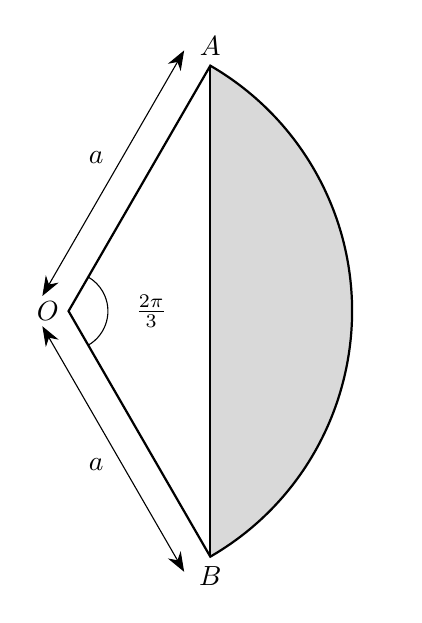
\begin{tikzpicture}[scale=1.2]
\def\rad{3}
\def\ang{60}
\def\dimoff{0.32}
\coordinate (O) at (0,0);
\coordinate (A) at (\ang:\rad);
\coordinate (B) at (-\ang:\rad);
\coordinate (OAstart) at ($(O)+({\ang+90}:\dimoff)$);
\coordinate (OAend) at ($(A)+({\ang+90}:\dimoff)$);
\coordinate (OBstart) at ($(O)+({-\ang-90}:\dimoff)$);
\coordinate (OBend) at ($(B)+({-\ang-90}:\dimoff)$);
\fill[gray!30] (B) arc[start angle=-\ang,end angle=\ang,radius=\rad] -- cycle;
\draw[thick,black] (O) -- (B) arc[start angle=-\ang,end angle=\ang,radius=\rad] -- cycle;
\draw[thick,black] (A) -- (B);
\pic["$\frac{2\pi}{3}$",draw,angle radius=5mm,angle eccentricity=2.1] {angle=B--O--A};
\draw[{Stealth[length=2.5mm]}-{Stealth[length=2.5mm]},black] (OAstart) -- (OAend) node[midway,above left] {$a$};
\draw[{Stealth[length=2.5mm]}-{Stealth[length=2.5mm]},black] (OBstart) -- (OBend) node[midway,below left] {$a$};
\node[left] at (O) {$O$};
\node[above] at (A) {$A$};
\node[below] at (B) {$B$};
\end{tikzpicture}
\end{figure}


A thin uniform metal plate has the shape of the shaded circular segment in the diagram above. \\
It is bounded by the chord $AB$ and the minor arc $AB$ of a circle with centre $O$ and radius $a$, where $a>0$. \\
The angle $AOB$ is $\frac{2\pi}{3}$. \\

The plate is modelled as a uniform lamina with constant mass per unit area $\sigma$, where $\sigma>0$. \\

Take $O$ as the origin and the positive $x$-axis along the bisector of angle $AOB$, directed towards the minor arc. \\
Thus the chord $AB$ lies on $x=\frac{a}{2}$. \\
\begin{enumerate}[label=\textbf{(\alph*)}]
\item Using integration, find the mass of the plate in terms of $\sigma$ and $a$. Give your answer in exact form. \marks{5} \\
\item Using integration to calculate the first moment of the plate about the $y$-axis, find the exact distance of its centre of mass from $O$. Explain why the centre of mass lies on the $x$-axis. \marks{5} \\
\end{enumerate}

\vspace*{10pt}

\begin{djsSolution}
\begin{enumerate}[label=\textbf{(\alph*)}, start=1]
\item
The upper endpoint \(A\) has height
\[
h=a\sin\left(\frac{\pi}{3}\right)=\frac{\sqrt{3}a}{2}
\]

Consider the region \(R_1\) between the curve \(x=\sqrt{a^2-y^2}\), the \(y\)-axis and the lines \(y=0\) and \(y=h\). The upper half of the plate is obtained by removing the rectangle \(R_2\), of width \(\frac{a}{2}\) and height \(h\), from \(R_1\).

For a region between a curve and the \(y\)-axis, the area formula gives
\[
\mathcal A_1=\int_0^h x\,\mathrm{d}y
=\int_0^h\sqrt{a^2-y^2}\,\mathrm{d}y
\]

Use \(y=a\sin t\), so \(\mathrm{d}y=a\cos t\,\mathrm{d}t\). The limits become \(t=0\) and \(t=\frac{\pi}{3}\), and \(\sqrt{a^2-y^2}=a\cos t\). Hence
\begin{align*}
\mathcal A_1
&=a^2\int_0^{\pi/3}\cos^2t\,\mathrm{d}t\\
&=\frac{a^2}{2}\int_0^{\pi/3}(1+\cos 2t)\,\mathrm{d}t\\
&=\frac{a^2}{2}\left[t+\frac{\sin 2t}{2}\right]_0^{\pi/3}\\
&=a^2\left(\frac{\pi}{6}+\frac{\sqrt{3}}{8}\right)
\end{align*}

The rectangle has area \(\mathcal A_2=\frac{ah}{2}=\frac{\sqrt{3}a^2}{4}\). Doubling the upper-half area and multiplying by the mass per unit area gives
\begin{align*}
M&=2\sigma(\mathcal A_1-\mathcal A_2)\\
&=2\sigma a^2\left(\frac{\pi}{6}+\frac{\sqrt{3}}{8}-\frac{\sqrt{3}}{4}\right)\\
&=\frac{\sigma a^2(4\pi-3\sqrt{3})}{12}
\end{align*}

\item
The plate is symmetric about the \(x\)-axis, so its centre of mass lies on that axis and \(\bar y=0\).

For a uniform lamina against the \(y\)-axis, the centre of mass formula is
\[
\bar{x}=\frac{1}{2\mathcal{A}}\int_c^d x^2\,\mathrm{d}y
\]

The rectangle \(R_2\) has \(\bar{x}_2=\frac{a}{4}\). For a uniform lamina made of pieces, the centre of mass formula is
\[
\bar{x}=\dfrac{\sum\mathcal{A}_i\bar{x}_i}{\sum\mathcal{A}_i}
\]

with the area of a removed piece counted as negative. Multiplied by \(\sigma\), its numerator is the first moment about the \(y\)-axis. Applying the formula for a lamina against the \(y\)-axis to \(R_1\), subtracting the rectangle's contribution and doubling to include the lower half gives
\begin{align*}
Q_y
&=2\sigma\left(\mathcal A_1\bar x_1-\mathcal A_2\bar x_2\right)\\
&=2\sigma\left(\frac12\int_0^h(a^2-y^2)\,\mathrm{d}y-\frac{ah}{2}\cdot\frac{a}{4}\right)\\
&=\sigma\left[a^2y-\frac{y^3}{3}\right]_0^h-\frac{\sigma a^2h}{4}\\
&=\sigma\left(\frac{3a^2h}{4}-\frac{h^3}{3}\right)\\
&=\sigma\left(\frac{3\sqrt{3}a^3}{8}-\frac{\sqrt{3}a^3}{8}\right)\\
&=\frac{\sqrt{3}\sigma a^3}{4}
\end{align*}

Since the plate lies to the right of \(O\), the required distance is \(\bar x\). Using the mass from part (a):
\[
\bar x=\frac{Q_y}{M}
=\frac{\dfrac{\sqrt{3}\sigma a^3}{4}}{\dfrac{\sigma a^2(4\pi-3\sqrt{3})}{12}}
=\frac{3\sqrt{3}a}{4\pi-3\sqrt{3}}
\]

\end{enumerate}
\end{djsSolution}

\newpage

% ---- Question 10 ----
\questionitem
% [Source: _QBT___Solns__Centre_of_Mass_of_Laminae_by_Integration, Q10]

\begin{figure}[H]
    \centering
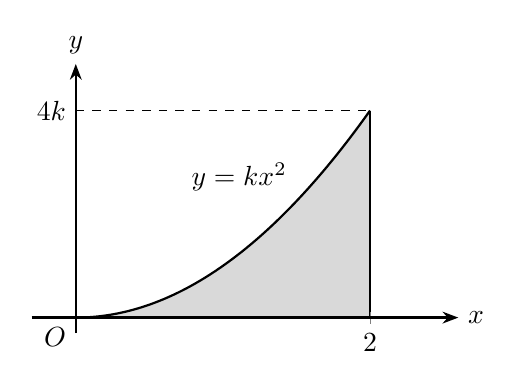
\begin{tikzpicture}
\def\k{1}
\def\extent{2}
\pgfmathsetmacro{\topheight}{\k*\extent^2}
\begin{axis}[axis lines=center,axis line style={thick,black,-{Stealth[length=2mm]}},xmin=-0.3,xmax=2.6,ymin=-0.3,ymax=4.9,width=7cm,height=5cm,xtick={2},ytick=\empty,xlabel={$x$},ylabel={$y$},every axis x label/.style={at={(ticklabel* cs:1)},anchor=west},every axis y label/.style={at={(ticklabel* cs:1)},anchor=south},axis on top,clip=true,clip mode=individual]
\addplot[draw=none,fill=gray!30,domain=0:\extent,samples=100] {\k*x^2} \closedcycle;
\addplot[thick,black,domain=0:\extent,samples=100] {\k*x^2};
\draw[thick,black] (axis cs:\extent,0) -- (axis cs:\extent,\topheight);
\draw[dashed,black] (axis cs:0,\topheight) -- (axis cs:\extent,\topheight);
\node[left] at (axis cs:0,\topheight) {$4k$};
\node[below left] at (axis cs:0,0) {$O$};
\node[above left] at (axis cs:1.5,{\k*1.5^2}) {$y=kx^2$};
\end{axis}
\end{tikzpicture}
\end{figure}


\begin{figure}[H]
    \centering
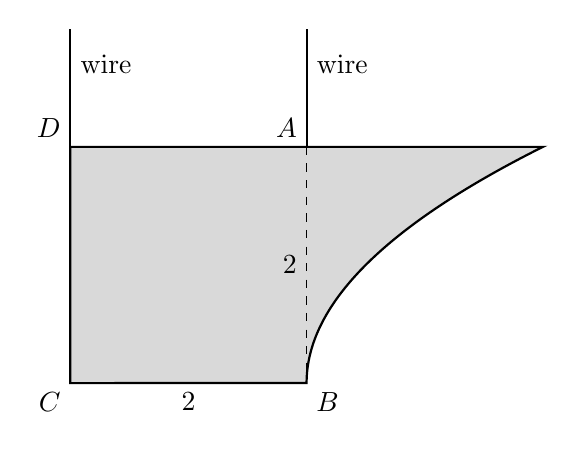
\begin{tikzpicture}[scale=1.5]
\def\k{0.5}
\def\width{2}
\def\height{2}
\def\wirelen{1.0}
\coordinate (C) at (0,0);
\coordinate (B) at (\width,0);
\coordinate (A) at (\width,\height);
\coordinate (D) at (0,\height);
\coordinate (E) at ({\width+\k*\height^2},\height);
\fill[gray!30] (D) -- (E) -- plot[domain=\height:0,samples=100,variable=\t] ({\width+\k*\t^2},\t) -- (C) -- cycle;
\draw[thick,black] (D) -- (E) -- plot[domain=\height:0,samples=100,variable=\t] ({\width+\k*\t^2},\t) -- (C) -- cycle;
\draw[dashed,black] (A) -- (B);
\foreach \P in {A,D} {
  \draw[thick,black] (\P) -- ++(0,\wirelen) node[pos=0.7,right] {wire};
}
\path (A) -- (B) node[midway,left] {$2$};
\path (C) -- (B) node[midway,below] {$2$};
\node[above left] at (A) {$A$};
\node[below right] at (B) {$B$};
\node[below left] at (C) {$C$};
\node[above left] at (D) {$D$};
\end{tikzpicture}
\end{figure}


A uniform lamina occupies the region bounded by the curve $y=kx^2$, the $x$-axis and the line $x=2$, where $k>0$, as shown in the first diagram above. \\
\begin{enumerate}[label=\textbf{(\roman*)}]
\item Use integration to find both coordinates of the centre of mass of this lamina in terms of $k$. \marks{8} \\
\end{enumerate}
A sign is made from a uniform sheet by joining a square $ABCD$ of side length $2$ to a curved piece having the shape of the lamina in part (i). \\
The sheet has the same thickness and density throughout. \\

For the sign, take $C$ as the origin, with $CB$ along the positive $x$-axis and $CD$ along the positive $y$-axis. \\
Thus $A=(2,2)$, $B=(2,0)$ and $D=(0,2)$. \\
The curved piece is obtained by reflecting the lamina in part (i) in the line $y=x$ and then translating it $2$ units to the right. \\
Its curved edge therefore has equation
\[
x=2+ky^2,\qquad 0\leq y\leq2
\] \\
The complete sign is shown in the second diagram above. \\
\begin{enumerate}[label=\textbf{(\roman*)}, resume]
\item Find both coordinates of the centre of mass of the sign in terms of $k$. \marks{5} \\
\end{enumerate}
The sign is held in equilibrium in a vertical plane by two vertical wires attached at $A$ and $D$. \\
The tension in the wire at $A$ is twice the tension in the wire at $D$. \\
\begin{enumerate}[label=\textbf{(\roman*)}, resume]
\item Find the exact value of $k$. \marks{5} \\
\end{enumerate}

\vspace*{10pt}

\begin{djsSolution}
\begin{enumerate}[label=\textbf{(\roman*)}, start=1]
\item
A vertical strip of width \(\mathrm{d}x\) under the curve has area \(y\,\mathrm{d}x\) and centre at \(\left(x,\frac12 y\right)\). For a uniform lamina under a curve, the centre of mass formulae are
\[
\mathcal{A}=\int_a^b y\,\mathrm{d}x,
\qquad
\bar{x}_L=\frac{1}{\mathcal{A}}\int_a^b xy\,\mathrm{d}x,
\qquad
\bar{y}_L=\frac{1}{2\mathcal{A}}\int_a^b y^2\,\mathrm{d}x
\]

Here \(y=kx^2\), with \(0\leq x\leq2\). The area is
\begin{align*}
\mathcal A
&=\int_0^2 kx^2\,\mathrm{d}x\\
&=k\left[\dfrac{x^3}{3}\right]_0^2
=\dfrac{8k}{3}
\end{align*}

Applying the centre of mass formulae:
\begin{align*}
\bar{x}_L
&=\dfrac{1}{8k/3}\int_0^2 kx^3\,\mathrm{d}x\\
&=\dfrac{k}{8k/3}\left[\dfrac{x^4}{4}\right]_0^2
=\dfrac{4k}{8k/3}
=\dfrac32\\
\bar{y}_L
&=\dfrac{1}{8k/3}\cdot\dfrac12\int_0^2 k^2x^4\,\mathrm{d}x\\
&=\dfrac{k^2}{2(8k/3)}\left[\dfrac{x^5}{5}\right]_0^2
=\dfrac{16k^2/5}{8k/3}
=\dfrac{6k}{5}
\end{align*}

\item
Reflection in \(y=x\) interchanges the centre's coordinates, and translation \(2\) units to the right adds \(2\) to its \(x\)-coordinate. Using part (i), the curved piece has area and centre
\[
\mathcal A_p=\dfrac{8k}{3},
\qquad
(\bar{x}_p,\bar{y}_p)=\left(2+\dfrac{6k}{5},\dfrac32\right)
\]

The square has area \(\mathcal A_s=4\) and centre \((\bar{x}_s,\bar{y}_s)=(1,1)\). Since the thickness and density are the same throughout, masses are proportional to areas. For a uniform lamina made of pieces, the centre of mass formulae are
\[
\bar{x}=\dfrac{\sum\mathcal{A}_i\bar{x}_i}{\sum\mathcal{A}_i},
\qquad
\bar{y}=\dfrac{\sum\mathcal{A}_i\bar{y}_i}{\sum\mathcal{A}_i}
\]

Summing over the square and the curved piece:
\begin{align*}
\bar{x}
&=\dfrac{4+\dfrac{8k}{3}\left(2+\dfrac{6k}{5}\right)}{4+\dfrac{8k}{3}}\\
&=\dfrac{4+\dfrac{16k}{3}+\dfrac{16k^2}{5}}{4+\dfrac{8k}{3}}
=\dfrac{12k^2+20k+15}{10k+15}\\
\bar{y}
&=\dfrac{4+\dfrac{8k}{3}\cdot\dfrac32}{4+\dfrac{8k}{3}}
=\dfrac{4+4k}{4+\dfrac{8k}{3}}
=\dfrac{3(k+1)}{2k+3}
\end{align*}

\item Let the tensions be \(T_A\) and \(T_D\), and let the sign's weight be \(W\). Vertical equilibrium gives
\[
W=T_A+T_D=2T_D+T_D=3T_D
\]

Taking moments about \(A\), the tension at \(D\) has horizontal distance \(2\), while the weight acts vertically through \(x=\bar{x}\). Thus
\begin{align*}
W(2-\bar{x})&=2T_D\\
3T_D(2-\bar{x})&=2T_D\\
2-\bar{x}&=\dfrac23\\
\bar{x}&=\dfrac43
\end{align*}

Using the \(x\)-coordinate from part (ii):
\begin{align*}
\dfrac{12k^2+20k+15}{10k+15}&=\dfrac43\\
3(12k^2+20k+15)&=4(10k+15)\\
36k^2+60k+45&=40k+60\\
36k^2+20k-15&=0\\
k&=\dfrac{-20\pm\sqrt{20^2-4(36)(-15)}}{72}\\
&=\dfrac{-5\pm4\sqrt{10}}{18}
\end{align*}

Since \(k>0\), the required value is
\[
k=\dfrac{4\sqrt{10}-5}{18}
\]

\end{enumerate}
\end{djsSolution}

\end{enumerate}
\end{document}
